\PassOptionsToPackage{naturalnames}{hyperref}
\RequirePackage{luatex85}
\documentclass{article}
\usepackage{geometry}
%\usepackage{fullpage}
\usepackage{parskip}
\usepackage{physics}
\usepackage{amsmath}
\usepackage{amssymb}
\usepackage{xcolor}
\usepackage[colorlinks,linkcolor=blue,citecolor=green]{hyperref}
\usepackage{array}
\usepackage{longtable}
\usepackage{multirow}
\usepackage{comment}
\usepackage{graphicx}
\usepackage{cite}
\usepackage{amsfonts}
\usepackage{bm}
\usepackage{slashed}
\usepackage{dsfont}
\usepackage{mathtools}
\usepackage[compat=1.1.0]{tikz-feynman}
\usepackage{simplewick}
%\usepackage{fourier}
%\usepackage{slashbox}
%\usepackage{intent}
\usepackage{mathrsfs}
\usepackage{xparse}
\usepackage{enumerate}
%\usepackage{axodraw4j}


\geometry{left=0.9cm,right=0.9cm,top=1.5cm,bottom=2cm}

\newcommand{\gm}{\gamma^{\mu}}
\newcommand{\gn}{\gamma^{\nu}}
\newcommand{\gs}{\gamma^{\sigma}}
\newcommand{\gr}{\gamma^{\rho}}
\newcommand{\gnr}{g^{\nu\rho}}
\newcommand{\gmr}{g^{\mu\rho}}
\newcommand{\gms}{g^{\mu\sigma}}
\newcommand{\gns}{g^{\nu\sigma}}
\newcommand{\vbp}{\vb{p}}
\newcommand{\vbk}{\vb{k}}
\newcommand{\g}{\gamma}
\renewcommand{\a}{\alpha}
\renewcommand{\b}{\beta}
\renewcommand{\t}{\theta}
\newcommand{\la}{\lambda}
\newcommand{\p}{\phi}
\newcommand{\vp}{\varphi}
\newcommand{\s}{\sigma}
\newcommand{\G}{\Gamma}
\newcommand{\pars}{\slashed\partial}
\newcommand{\ps}{\slashed p}
\newcommand{\ks}{\slashed k}
\newcommand{\lag}{\mathcal{L}}
\newcommand{\da}{^{\dagger}}
\newcommand{\sm}{^{\mu}}
\newcommand{\sn}{^{\nu}}
\newcommand{\smn}{^{\mu\nu}}
\newcommand{\Dm}{D^{\mu}}
\newcommand{\dm}{\partial^{\mu}}
\newcommand{\Asquare}{A^{\mu}A_{\mu}}
\newcommand{\partialsquare}[2]{\partial^{\mu}{#1}\partial_{\mu}{#2}}

\title{Hydrogen}
\author{Yingsheng Huang}
\begin{document}
\maketitle
\section{Matching}
QED Lagrangian is
\begin{align}
  \lag_{QED}=\bar l(i\slashed D-m)l+\bar N(i D^0)N-\lag_{\gamma}
  \label{}
\end{align}
Set the NRQED Lagrangian as (take large $M$ limit where $M$ is the mass of the proton/hydrogen nucleus)
\begin{align}
  \lag_{NRQED}=\psi^{\dagger}(iD_0+\frac{\vb{D}^2}{2m})\psi+\bar N(iD_0)N+\lag_{4-fer}+\lag_{\gamma}
  \label{}
\end{align}
In tree level\footnote{Note that there's no Gamma matrice in the heavy particle side, they can only appear in the QED side. }
\begin{align*}
  i\mathcal{M}_{QED}^{(0)}&=\feynmandiagram[horizontal=i1 to f1,layered layout,inline=($(a)!0.5!(c)$),medium]{
	i1[particle=$P_N$] -- [double distance=1pt] a -- [double distance=1pt] f1[particle=$P_N$],
	i2[particle=$p_1$] -- [fermion] c -- [fermion] f2[particle=$p_2$],
	{ [same layer] a -- [photon,momentum'=$q$] c},
  };=-e^2\bar u_N(P_N)v^{0}u_N(P_N)\frac{i}{\vb{q}^2}\bar u_e(p_2)\g_{0}u_e(p1)
\end{align*}
\begin{align*}
  i\mathcal{M}_{NRQED}^{(0)}&=\feynmandiagram[horizontal=i1 to f1,layered layout,inline=($(a)!0.5!(c)$),medium]{
	i1[particle=$P_N$] -- [double distance=1pt] a -- [double distance=1pt] f1[particle=$P_N$],
	i2[particle=$p_1$] -- [fermion] c -- [fermion] f2[particle=$p_2$],
	{ [same layer] a -- [photon,momentum'=$q$] c},
  };=-e^2\bar u_N(P_N)v^{0}u_N(P_N)\frac{i}{\vb{q}^2}\psi^{\dagger}(p_2)\psi(p1)
\end{align*}

The box %and crossed box
diagram for NRQED process is
\begin{align*}
  i\mathcal{M}_{NRQED}^{(1)}&=\feynmandiagram[horizontal=i1 to f1,layered layout,inline=($(a)!0.5!(c)$),medium]{
	i1[particle=$P_N$] -- [double distance=1pt] a -- [double distance=1pt,momentum=$P_N-k$] b -- [double distance=1pt] f1[particle=$P_N$],
	i2[particle=$p_1$] -- [fermion] c -- [fermion,momentum'=$p1+k$] d -- [fermion] f2[particle=$p_2$],
	{ [same layer] a -- [photon,momentum'=$k$] c},
	{ [same layer] b-- [photon,rmomentum=$k-q$] d},
  };\\
  &=e^4\bar u_N(P_N)\frac{1+\g^0}{2}u_N(P_N)\psi^{\dagger}(p_2)\int[\dd k]\frac{1}{\vb{k}^2(\vb{k}-\vb{q})^2(-k^0+i\epsilon)(p_1^0+k^0-m-\frac{\vb{(p_1+k)}^2}{2m}+i\epsilon)}\psi(p_1)\\
  &=-ie^4\bar u_N(P_N)\frac{1+\g^0}{2}u_N(P_N)\psi^{\dagger}(p_2)\int\frac{\dd^3k}{(2\pi)^3}\frac{1}{\vb{k}^2(\vb{k}-\vb{q})^2(E_1-\frac{\vb{(p_1+k)}^2}{2m})}\psi(p_1)\\
  &=-ie^4\bar u_N(P_N)\frac{1+\g^0}{2}u_N(P_N)\psi^{\dagger}(p_2)\int\frac{\dd^3k}{(2\pi)^3}\frac{1}{(\vb{k}-\vb{p_1})^2(\vb{k}-\vb{p_2})^2(E_1-\frac{\vb{k}^2}{2m})}\psi(p_1)
\end{align*}
%\clearpage
The box and crossed box diagram for QED process is
\begin{align*}
  i\mathcal{M}_1^{(1)}&=\feynmandiagram[horizontal=i1 to f1,layered layout,inline=($(a)!0.5!(c)$),medium]{
	i1[particle=$P_N$] -- [double distance=1pt] a -- [double distance=1pt,momentum=$P_N-k$] b -- [double distance=1pt] f1[particle=$P_N$],
	i2[particle=$p_1$] -- [fermion] c -- [fermion,momentum'=$p1+k$] d -- [fermion] f2[particle=$p_2$],
	{ [same layer] a -- [photon,momentum'=$k$] c},
	{ [same layer] b-- [photon,rmomentum=$k-q$] d},
  };\\
  &=e^4\bar u_N(P_N)\frac{1+\g^0}{2}u_N(P_N)u_e^{\dagger}(p_2)\int[\dd k]\frac{(\slashed p_1+\slashed k+m)\g^0}{\vb{k}^2(\vb{k}-\vb{q})^2[(p_1+k)^2-m^2+i\epsilon](-k^0+i\epsilon)}u_e(p_1)\\
  &=e^4\bar u_N(P_N)\frac{1+\g^0}{2}u_N(P_N)u_e^{\dagger}(p_2)\int[\dd k]\frac{2p_1^0+\slashed k\g^0}{\vb{k}^2(\vb{k}-\vb{q})^2[(p_1+k)^2-m^2+i\epsilon](-k^0+i\epsilon)}u_e(p_1)\\
  &=ie^4\bar u_N(P_N)\frac{1+\g^0}{2}u_N(P_N)u_e^{\dagger}(p_2)\int\frac{\dd^3 k}{(2\pi)^3}\frac{p_1^0+k_i\g^i\g^0+\sqrt{(\vb{k}+\vb{p_1})^2+m^2}}{2\vb{k}^2(\vb{k}-\vb{q})^2[(\vb{k}+\vb{p_1})^2+m^2-p_1^0\sqrt{(\vb{k}+\vb{p_1})^2+m^2}]}u_e(p_1)\\
  &=ie^4\bar u_N(P_N)\frac{1+\g^0}{2}u_N(P_N)u_e^{\dagger}(p_2)\int\frac{\dd^3 k}{(2\pi)^3}\frac{p_1^0+(k_i-p_{1i})\g^i\g^0+\sqrt{\vb{k}^2+m^2}}{2(\vb{k}-\vb{p_1})^2(\vb{k}-\vb{p_2})^2[\vb{k}^2+m^2-p_1^0\sqrt{\vb{k}^2+m^2}]}u_e(p_1)
 \end{align*}
 $i\mathcal{M}_1^{(1)}$ has infrared log divergence and no ultraviolet divergence.
 \begin{align*}
  i\mathcal{M}_2^{(1)}&=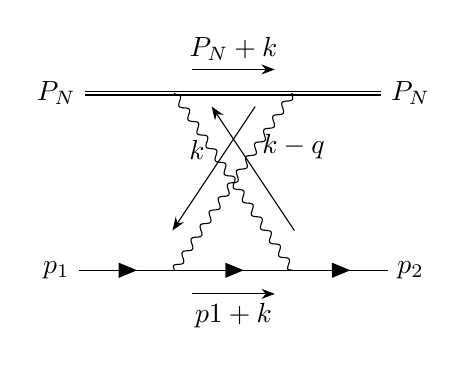
\begin{tikzpicture}[baseline=($(a)!0.5!(c)$)]
	\begin{feynman}
	  \diagram[horizontal=i1 to f1,layered layout,medium]{
		i1[particle=$P_N$] -- [double distance=1pt] a -- [double distance=1pt,momentum=$P_N+k$] b -- [double distance=1pt] f1[particle=$P_N$],
	i2[particle=$p_1$] -- [fermion] c -- [fermion,momentum'=$p1+k$] d -- [fermion] f2[particle=$p_2$],
	{ [same layer] a --[draw=none] c},
	{ [same layer] b-- [draw=none] d},
  };
	  \diagram*{
		(a) -- [photon,rmomentum=$k-q$] (d),
		(b) -- [photon,momentum'=$k$] (c),
	  };
	\end{feynman}
  \end{tikzpicture}\\
  &=e^4\bar u_N(P_N)\frac{1+\g^0}{2}u_N(P_N)u_e^{\dagger}(p_2)\int[\dd k]\frac{(\slashed p_1+\slashed k+m)\g^0}{\vb{k}^2(\vb{k}-\vb{q})^2[(p_1+k)^2-m^2+i\epsilon](k^0+i\epsilon)}u_e(p_1)\\
  &=e^4\bar u_N(P_N)\frac{1+\g^0}{2}u_N(P_N)u_e^{\dagger}(p_2)\int[\dd k]\frac{2p_1^0+\slashed k\g^0}{\vb{k}^2(\vb{k}-\vb{q})^2[(p_1+k)^2-m^2+i\epsilon](k^0+i\epsilon)}u_e(p_1)\\
  &=-ie^4\bar u_N(P_N)\frac{1+\g^0}{2}u_N(P_N)u_e^{\dagger}(p_2)\int\frac{\dd^3 k}{(2\pi)^3}\frac{p_1^0+k_i\g^i\g^0-\sqrt{(\vb{k}+\vb{p_1})^2+m^2}}{2\vb{k}^2(\vb{k}-\vb{q})^2[(\vb{k}+\vb{p_1})^2+m^2+p_1^0\sqrt{(\vb{k}+\vb{p_1})^2+m^2}]}u_e(p_1)\\
  &=-ie^4\bar u_N(P_N)\frac{1+\g^0}{2}u_N(P_N)u_e^{\dagger}(p_2)\int\frac{\dd^3 k}{(2\pi)^3}\frac{p_1^0+(k_i-p_{1i})\g^i\g^0-\sqrt{\vb{k}^2+m^2}}{2(\vb{k}-\vb{p_1})^2(\vb{k}-\vb{p_2})^2[\vb{k}^2+m^2+p_1^0\sqrt{\vb{k}^2+m^2}]}u_e(p_1)
 \end{align*}
 $i\mathcal{M}_2^{(1)}$ has no infrared or ultraviolet divergence.
%\includegraphics[width=0.5\textwidth]{NRQED.eps}
 \begin{align*}
 i\mathcal{M}_1^{(1)}+i\mathcal{M}_2^{(1)}&=ie^4\bar u_N(P_N)\frac{1+\g^0}{2}u_N(P_N)u_e^{\dagger}(p_2)\int\frac{\dd^3 k}{(2\pi)^3}\frac{{p_1^0}^2+k^2+m^2+(k_i-p_{1i})p_1^0\g^i\g^0}{(\vb{k}-\vb{p_1})^2(\vb{k}-\vb{p_2})^2[\vb{k}^2+m^2-{p_1^0}^2]\sqrt{\vb{k}^2+m^2}}u_e(p_1)\\
 &=ie^4\bar u_N(P_N)\frac{1+\g^0}{2}u_N(P_N)u_e^{\dagger}(p_2)\int\frac{\dd^3 k}{(2\pi)^3}\frac{{p_1^0}^2+k^2+m^2+(k_i-p_{1i})p_1^0\g^i\g^0}{(\vb{k}-\vb{p_1})^2(\vb{k}-\vb{p_2})^2[\vb{k}^2-\vb{p_1}^2]\sqrt{\vb{k}^2+m^2}}u_e(p_1)
 \end{align*}
 Note that after the expansion over external momentum, $k^i$ can be converted into $p^i$ so it's actually at $p^1$ order.

 Now consider operator product expansion.

 Tree level matching: 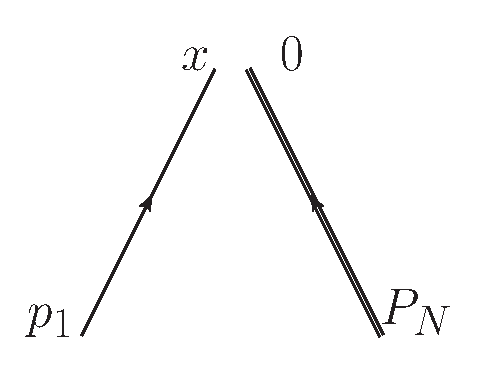
\includegraphics[width=1.2 in]{OPE-00.eps} \& 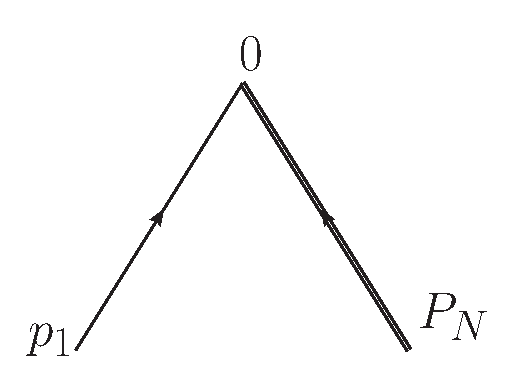
\includegraphics[width=1.2 in]{OPE-0.eps}

 \begin{align*}
   &\mel{0}{T\psi(x)N(0)}{pP_N} = 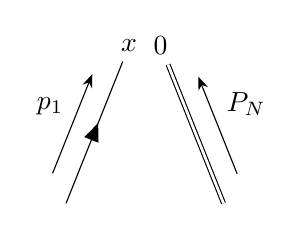
\begin{tikzpicture}[baseline=($(p1)!0.5!(x)$)]
	\begin{feynman}
    \vertex (p1);
	\vertex[right=2cm of p1] (p2);
	\vertex at ($(p1)!0.4!(p2)+(0,2cm)$) (x) {$x$};
	\vertex at ($(p1)!0.6!(p2)+(0,2cm)$) (0) {$0$};
	%
	\diagram* {
      (p1) -- [momentum=\(p_{1}\), fermion] (x);
	  (p2) -- [momentum'=\(P_{N}\), double distance=1pt] (0);
    };
  \end{feynman}
\end{tikzpicture}= u_e(p)u_N(P_N)e^{-ip\cdot x}\\
   &\mel{0}{T\psi_e(x)N(0)}{pP_N} = 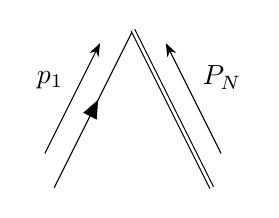
\begin{tikzpicture}[baseline=($(p1)!0.5!(x)$)]
	\begin{feynman}
    \vertex (p1);
	\vertex[right=2cm of p1] (p2);
	\vertex at ($(p1)!0.5!(p2)+(0,2cm)$) (x);
	%
	\diagram* {
	  (p1) -- [momentum=\(p_{1}\), fermion] (x) [particle=$0$];
	  (p2) -- [momentum'=\(P_{N}\), double distance=1pt] (x);
    };
  \end{feynman}
\end{tikzpicture}=\psi_e(p)u_N(P_N)
\end{align*}
At leading order $u_e(p)=\pmqty{\psi_e(p)\\0}$. (If we're only interested in the hard region contribution, which is independent of states, the leading order is independent of any on-shell momentums.)

%\begin{align*}

%\end{align*}

 One loop scenario for NRQED case:
 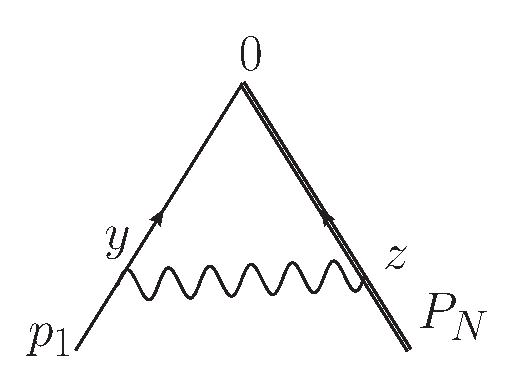
\includegraphics[width=1.2 in]{OPE-1.eps}
 \begin{align*}
    \mel{0}{\psi_e(0)N(0)e\int\dd^4y\bar\psi_e\psi_e A^0e\int\dd^4z\bar NNA^0}{eN}&=e^2u_N(v_N)\int[\dd k]\frac{1}{\vb{k}^2(-k^0+i\epsilon)(p_1^0+k^0-m-\frac{\vb{(p_1+k)}^2}{2m}+i\epsilon)}\psi(p_1)\\
  &=-ie^2u_N(v_N)\int\frac{\dd^3k}{(2\pi)^3}\frac{1}{\vb{k}^2(E_1-\frac{\vb{(p_1+k)}^2}{2m}+i\epsilon)}\psi(p_1)\\
  &=-ie^2u_N(v_N)\int\frac{\dd^3k}{(2\pi)^3}\frac{1}{(\vb{k}-\vb{p_1})^2(E_1-\frac{\vb{k}^2}{2m}+i\epsilon)}\psi(p_1)\\
  \intertext{drop $p_1$}
  &=-ie^2u_N(v_N)\int\frac{\dd^3k}{(2\pi)^3}\frac{1}{\vb{k}^2(E_1-\frac{\vb{k}^2}{2m}+i\epsilon)}\psi(p_1)=\pi ie^2\sqrt{\frac{2m}{E_1}}u_N(v_N)\psi(p_1)
 \end{align*}
For QED case:
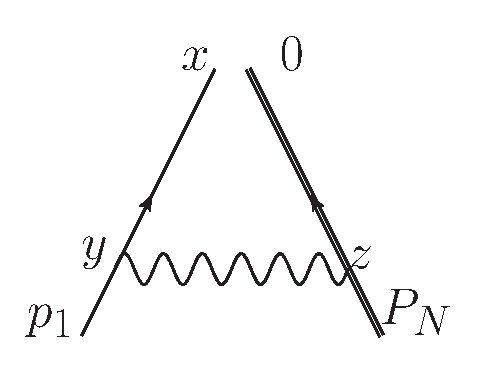
\includegraphics[width=1.2 in]{OPE-2.eps}
\begin{align*}
  \mel{0}{\psi(x)N(0)e\int\dd^4y\bar\psi\g^0\psi A^0 e\int\dd^4 z \bar N NA^0}{eN}\text{\footnotemark}&=e^2u_N(v_N)\int[\dd k]e^{-i\vb{(k+p_1)}\cdot\vb{x}}\frac{(\slashed p_1+\slashed k+m)\g^0}{\vb{k}^2[(p_1+k)^2-m^2+i\epsilon](-k^0+i\epsilon)}u_e(p_1)\\
  &=e^2u_N(v_N)\int[\dd k]e^{-i\vb{(k+p_1)}\cdot\vb{x}}\frac{2p_1^0+\slashed k\g^0}{\vb{k}^2[(p_1+k)^2-m^2+i\epsilon](-k^0+i\epsilon)}u_e(p_1)\\
  &=ie^2u_N(v_N)\int\frac{\dd^3 k}{(2\pi)^3}e^{-i\vb{(k+p_1)}\cdot\vb{x}}\frac{p_1^0+k_i\g^i\g^0+\sqrt{(\vb{k}+\vb{p_1})^2+m^2}}{2\vb{k}^2[(\vb{k}+\vb{p_1})^2+m^2-p_1^0\sqrt{(\vb{k}+\vb{p_1})^2+m^2}]}u_e(p_1)\\
  &=ie^2u_N(v_N)\int\frac{\dd^3 k}{(2\pi)^3}e^{-i\vb{k}\cdot\vb{x}}\frac{p_1^0+(k_i-p_{1i})\g^i\g^0+\sqrt{\vb{k}^2+m^2}}{2(\vb{k}-\vb{p_1})^2[\vb{k}^2+m^2-p_1^0\sqrt{\vb{k}^2+m^2}]}u_e(p_1)\\
  \intertext{drop $\vb{p_1}$}
  &=ie^2u_N(v_N)\int\frac{\dd^3 k}{(2\pi)^3}e^{-i\vb{k}\cdot\vb{x}}\frac{p_1^0+\sqrt{\vb{k}^2+m^2}}{2\vb{k}^2[\vb{k}^2+m^2-p_1^0\sqrt{\vb{k}^2+m^2}]}u_e(p_1)
\end{align*}%\addtocounter{footnote}{-1}\stepcounter{footnote}
 \footnotetext{$\mel{0}{\psi(x)N(0)e\int\dd^4y\bar\psi\g^0\psi A^0 e\int\dd^4 z \bar N NA^0}{eN}=e^2\int\dd^4y\int\dd^4z\int\frac{\dd^4k}{(2\pi)^4}\frac{i}{\vb{k^2}}e^{-ik\cdot(z-y)}\int\frac{\dd^4k_1}{(2\pi)^4}\tilde S_e(k_1)e^{-ik_1\cdot(y-x)}\int\frac{\dd^4k_2}{(2\pi)^4}\tilde S_N(k_2)u_N(v_N)u_e(p)e^{-ip_1\cdot y}$.}

 Two loop scenario for QED case $\mel{0}{T\psi(x)N(0)e\int\dd^4y_1\bar\psi\g^0\psi A^0 e\int\dd^4 z_1 \bar N NA^0e\int\dd^4y_2\bar\psi\g^0\psi A^0 e\int\dd^4 z_2 \bar N NA^0}{eN}$:
 \begin{align*}
   &-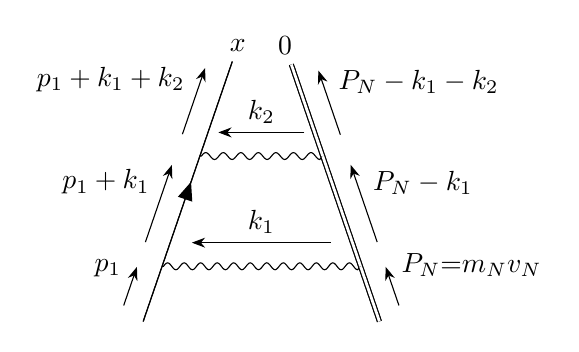
\begin{tikzpicture}[baseline=($(p1)!0.5!(x)$)]
	\begin{feynman}
    \vertex (p1);
	\vertex[right=3cm of p1] (p2);
	\vertex at ($(p1)!0.4!(p2)+(0,3.5cm)$) (x) {$x$};
	\vertex at ($(p1)!0.6!(p2)+(0,3.5cm)$) (0) {$0$};
	\vertex at ($(p1)!0.2!(x)$) (y1);
	\vertex at ($(p2)!0.2!(0)$) (z1);
	\vertex at ($(p1)!0.6!(x)$) (y2);
	\vertex at ($(p2)!0.6!(0)$) (z2);
	%
	\diagram* {
	  (p1) -- [fermion] (x);
	  (p2) -- [double distance=1pt] (0);
	  (y1) -- [photon,rmomentum=$k_1$] (z1);
	  (y2) -- [photon,rmomentum=$k_2$] (z2);
	  (p1) -- [momentum=\(p_{1}\)] (y1);
	  (p2) -- [momentum'=$P_{N}\text{=}m_{N}v_{N}$,double distance=1pt] (z1);
	  (y1) -- [momentum=\(p_{1}+k_1\)] (y2);
	  (z1) -- [momentum'=\(P_{N}-k_1\),double distance=1pt] (z2);
	  (y2) -- [momentum=\(p_{1}+k_1+k_2\)] (x);
	  (z2) -- [momentum'=\(P_{N}-k_1-k_2\),double distance=1pt] (0);
    };
	\end{feynman}
  \end{tikzpicture}
  \\
  =&e^4\int[dk_1][dk_2]e^{-i\vb{(p_1+k_1+k_2)}\vdot \vb{x}}\frac{1}{\vb{\abs{k_1}}^2}\frac{1}{\vb{\abs{k_2}}^2}\frac{1}{-k_1^0-k_2^0+i\epsilon}\frac{1}{-k_1^0+i\epsilon}\frac{\slashed p_1+\slashed k_1+\slashed k_2+m}{(p_1+ k_1+ k_2)^2-m^2+i\epsilon}\g^0\frac{\slashed p_1+\slashed k_1+m}{(p_1+ k_1)^2-m^2+i\epsilon}\g^0u_N(v_N)u_e(p_1)\\
  =&e^4\int[dk_1][dk_2]e^{-i\vb{(p_1+k_1+k_2)}\vdot \vb{x}}\frac{1}{\vb{\abs{k_1}}^2\vb{\abs{k_2}}^2}
  \frac{4{p_1^0}^2+2p_1^0k_1^0+2\vb{p_1}\cdot\vb{k_1}+2(p_1^0+k_1^0)(\slashed k_1+\slashed k_2)\g^0-\slashed k_2\slashed k_1}{\bqty{(p_1+ k_1+ k_2)^2-m^2+i\epsilon}\bqty{(p_1+ k_1)^2-m^2+i\epsilon}\bqty{-k_1^0-k_2^0+i\epsilon}\bqty{-k_1^0+i\epsilon}}
  u_N(v_N)u_e(p_1)\footnotemark\\
  =&ie^4\int[\dd k_1]\frac{\dd^3\vb{k_2}}{(2\pi)^3}
  \frac{2(k_1^0+p_1^0)[(\sqrt{(\vb{p_1+k_1+k_2})^2+m^2}-k_1^0-p_1^0)+(k_2^i\g_i+\slashed k_1)\g^0]-[\g^0(\sqrt{(\vb{p_1+k_1+k_2})^2+m^2}-k_1^0-p_1^0)-k_2^i\g_i]\slashed k_1}{2\sqrt{(\vb{p_1+k_1+k_2})^2+m^2}(\sqrt{(\vb{p_1+k_1+k_2})^2+m^2}-k_1^0+\frac{ 2 ((\vb{p_1+k_1+k_2})^2+m^2)+2 \sqrt{(\vb{p_1+k_1+k_2})^2+m^2}-p_1^0}{2 ((\vb{p_1+k_1+k_2})^2+m^2)}i \epsilon )}\\&
  \frac{1}{-k_1^0+i\epsilon}\frac{1}{(p_1+ k_1)^2-m^2+i\epsilon}\frac{1}{\vb{\abs{k_1}}^2\vb{\abs{k_2}}^2}u_N(v_N)u_e(p_1)e^{-i\vb{(p_1+k_1+k_2)}\vdot \vb{x}}\\
  \intertext{define $a=(\vb{p_1+k_1+k_2})^2+m^2$ and $b=\sqrt{(\vb{p_1+k_1+k_2})^2+m^2}-k_1^0-p_1^0+k_2^i\g_i\g^0=\sqrt{a}-k_1^0-p_1^0+k_2^i\g_i\g^0$ (pole location is $\sqrt{a}-k_1^0-p_1^0-\frac{i\epsilon}{2\sqrt{a}}$), and note that the long coefficient of the first $\epsilon$ above is positive}
  =&ie^4\int[\dd k_1]\frac{\dd^3\vb{k_2}}{(2\pi)^3}
  \frac{2(k_1^0+p_1^0)[b+\slashed k_1\g^0]-\g^0b\slashed k_1}{2\sqrt{a}(\sqrt{a}-k_1^0+i \epsilon )}
  \frac{1}{-k_1^0+i\epsilon}\frac{1}{(p_1+ k_1)^2-m^2+i\epsilon}\frac{1}{\vb{\abs{k_1}}^2\vb{\abs{k_2}}^2}u_N(v_N)u_e(p_1)e^{-i\vb{(p_1+k_1+k_2)}\vdot \vb{x}}\\
  \intertext{also define $b'$ so that $b=b'-k_1^0$ ($b'=\sqrt{a}-p_1^0+k_2^i\g_i\g^0$) and $a'=(\vb{p_1+k_1})^2+m^2$}
  =&ie^4\int[\dd k_1]\frac{\dd^3\vb{k_2}}{(2\pi)^3}
  \frac{2(k_1^0+p_1^0)[b'+k_1^i\g_i\g^0]-\g^0(b'-k_1^0)(k_1^0\g^0+ k_1^i\g_i)}{2\sqrt{a}(\sqrt{a}-k_1^0+i \epsilon )\bqty{-k_1^0+i\epsilon}}
  \frac{1}{(p_1+ k_1)^2-m^2+i\epsilon}\frac{1}{\vb{\abs{k_1}}^2\vb{\abs{k_2}}^2}u_N(v_N)u_e(p_1)e^{-i\vb{(p_1+k_1+k_2)}\vdot \vb{x}}\\
  =&-e^4\int\frac{\dd^3\vb{k_1}}{(2\pi)^3}\frac{\dd^3\vb{k_2}}{(2\pi)^3}
  \frac{2\sqrt{a'}(b'+k_1^i\g_i\g^0)+\g^0(\sqrt{a'}-b'-p_1^0)(\sqrt{a'}\g^0-p_1^0\g^0+k_1^i\g_i)}{4\sqrt{a}\sqrt{a'}(\sqrt{a'}-p_1^0)(\sqrt{a}-\sqrt{a'}+p_1^0)}
  \frac{1}{\vb{\abs{k_1}}^2\vb{\abs{k_2}}^2}u_N(v_N)u_e(p_1)e^{-i\vb{(p_1+k_1+k_2)}\vdot \vb{x}}\\
  \intertext{shift both loop momentum\footnotemark{} so that $a=\abs{\vb{k_2}}^2+m^2$ and $a'=\abs{\vb{k_1}}^2+m^2$, now $b=\sqrt{a}-k_1^0+(k_2-k_1)^i\g_i\g^0$ and $b'=\sqrt{a}+(k_2-k_1)^i\g_i\g^0$}
  =&-e^4\int\frac{\dd^3\vb{k_1}}{(2\pi)^3}\frac{\dd^3\vb{k_2}}{(2\pi)^3}
  \frac{2\sqrt{a'}(\sqrt{a}+(k_2-p_1)^i\g_i\g^0)+(\sqrt{a'}-\sqrt{a}+(k_2-k_1)^i\g_i\g^0-p_1^0)(\sqrt{a'}-p_1^0-(k_1-p_1)^i\g_i\g^0)}{4\sqrt{a}\sqrt{a'}(\sqrt{a'}-p_1^0)(\sqrt{a}-\sqrt{a'}+p_1^0){\vb{\abs{k_1-p_1}}^2\vb{\abs{k_2-k_1}}^2}}
  u_N(v_N)u_e(p_1)e^{-i\vb{k_2}\vdot \vb{x}}\\
  \intertext{drop $\vb{p_1}$}
  =&-e^4\int\frac{\dd^3\vb{k_1}}{(2\pi)^3}\frac{\dd^3\vb{k_2}}{(2\pi)^3}
  \frac{2\sqrt{a'}(\sqrt{a}+k_2^i\g_i\g^0)+(\sqrt{a'}-\sqrt{a}+(k_2-k_1)^i\g_i\g^0-p_1^0)(\sqrt{a'}-p_1^0-k_1^i\g_i\g^0)}{4\sqrt{a}\sqrt{a'}(\sqrt{a'}-p_1^0)(\sqrt{a}-\sqrt{a'}+p_1^0){\vb{\abs{k_1}}^2\vb{\abs{k_2-k_1}}^2}}
  u_N(v_N)u_e(p_1)e^{-i\vb{k_2}\vdot \vb{x}}\\
  \intertext{rewrite it with $a_1=a'$ and $a_2=a$}
   =&-e^4\int\frac{\dd^3\vb{k_1}}{(2\pi)^3}\frac{\dd^3\vb{k_2}}{(2\pi)^3}
    \frac{2\sqrt{a_1}(\sqrt{a_2}+k_2^i\g_i\g^0)+(\sqrt{a_1}-\sqrt{a_2}+(k_2-k_1)^i\g_i\g^0-p_1^0)(\sqrt{a_1}-p_1^0-k_1^i\g_i\g^0)}{4\sqrt{a_1}\sqrt{a_2}(\sqrt{a_1}-p_1^0)(\sqrt{a_2}-\sqrt{a_1}+p_1^0){\vb{\abs{k_1}}^2\vb{\abs{k_2-k_1}}^2}}
    u_N(v_N)u_e(p_1)e^{-i\vb{k_2}\vdot \vb{x}}\\
  \intertext{to investigate the divergent property of the integral, rewrite the integral before the shift ($a_1=\pqty{\vb{p_1+k_1}}^2+m^2$ and $a_2=\pqty{\vb{p_1+k_1+k_2}}^2+m^2$)}
  =&-e^4\int\frac{\dd^3\vb{k_1}}{(2\pi)^3}\frac{\dd^3\vb{k_2}}{(2\pi)^3}
  \frac{2\sqrt{a_1}(\sqrt{a_2}-p_1^0+(k_1+k_2)^i\g_i\g^0)+(\sqrt{a_1}-\sqrt{a_2}+k_2^i\g_i\g^0)(\sqrt{a_1}-p_1^0-k_1^i\g_i\g^0)}{4\sqrt{a_1}\sqrt{a_2}(\sqrt{a_1}-p_1^0)(\sqrt{a_2}-\sqrt{a_1}+p_1^0){\vb{\abs{k_1}}^2\vb{\abs{k_2}}^2}}
  u_N(v_N)u_e(p_1)e^{-i\vb{(p_1+k_1+k_2)}\vdot \vb{x}}
%  =&ie^4\int[\dd k_1]\frac{\dd^3\vb{k_2}}{(2\pi)^3}\frac{4m^2+2k_1\cdot p_1-(\slashed k_1+2m)(-\sqrt{(\vb{p_1+k_1+k_2})^2+m^2}+k_1^0+p_1^0)\g^0+(\slashed k_1+2m)k_2^i\g_i}{2\sqrt{(\vb{p_1+k_1+k_2})^2+m^2}(\sqrt{(\vb{p_1+k_1+k_2})^2+m^2}-k_1^0+\frac{ 2 ((\vb{p_1+k_1+k_2})^2+m^2)+2 \sqrt{(\vb{p_1+k_1+k_2})^2+m^2}-p_1^0}{2 ((\vb{p_1+k_1+k_2})^2+m^2)}i \epsilon )}\\&\frac{1}{\vb{\abs{k_1}}^2}\frac{1}{\vb{\abs{k_2}}^2}\frac{1}{-k_1^0+i\epsilon}\frac{1}{(p_1+ k_1)^2-m^2+i\epsilon}u_N(v_N)u_e(p_1)e^{-i\vb{(p_1+k_1+k_2)}\vdot \vb{x}}\\
%  \intertext{note that the long coefficient of the first $\epsilon$ above is positive}
%  =&ie^4\int[\dd k_1]\frac{\dd^3\vb{k_2}}{(2\pi)^3}\frac{4m^2+2k_1\cdot p_1-(\slashed k_1+2m)(-\sqrt{(\vb{p_1+k_1+k_2})^2+m^2}+k_1^0+p_1^0)\g^0+(\slashed k_1+2m)k_2^i\g_i}{2\sqrt{(\vb{p_1+k_1+k_2})^2+m^2}(\sqrt{(\vb{p_1+k_1+k_2})^2+m^2}-k_1^0+i \epsilon )}\\&\frac{1}{\vb{\abs{k_1}}^2}\frac{1}{\vb{\abs{k_2}}^2}\frac{1}{-k_1^0+i\epsilon}\frac{1}{(p_1+ k_1)^2-m^2+i\epsilon}u_N(v_N)u_e(p_1)e^{-i\vb{(p_1+k_1+k_2)}\vdot \vb{x}}\\
  %=&e^4\int\frac{\dd^3\vb{k_1}}{(2\pi)^3}\frac{\dd^3\vb{k_2}}{(2\pi)^3}\frac{k_2^i {\gamma }_i \left({\gamma }^0 \left(\sqrt{(\vb{p_1+k_1+k_2})^2+m^2}-p_1^0\right)+2 m\right)+k_1^i k_2^j \g_i\g_j-2 \left(-\sqrt{(\vb{p_1+k_1+k_2})^2+m^2} p_1^0+\vb{k_1}\cdot \vb{p_1}+{p_1^0}^2\right)+4 m^2}{4 ((\vb{p_1+k_1+k_2})^2+m^2) p_1^0 \left(\sqrt{(\vb{p_1+k_1+k_2})^2+m^2}-p_1^0\right)}\\&\frac{1}{\vb{\abs{k_1}}^2}\frac{1}{\vb{\abs{k_2}}^2}u_N(v_N)u_e(p_1)e^{-i\vb{(p_1+k_1+k_2)}\vdot \vb{x}}\\
 \end{align*}
 \addtocounter{footnote}{-1}\footnotetext{With a $u_e(p_1)$ on the right hand side, $(\slashed p_1+\slashed k_1+\slashed k_2+m)\g^0(\slashed p_1+\slashed k_1+m)\g^0=(\slashed p_1+\slashed k_1+\slashed k_2+m)[2(p_1^0+k_1^0)\g^0-(\slashed p_1+\slashed k_1-m)]=2(p_1^0+k_1^0)(\slashed p_1+\slashed k_1+\slashed k_2+m)\g^0-(\slashed p_1+\slashed k_1+\slashed k_2+m)(\slashed p_1+\slashed k_1-m)=2(p_1^0+k_1^0)(\slashed p_1+\slashed k_1+\slashed k_2+m)\g^0-(\slashed p_1+\slashed k_1+\slashed k_2+m)\slashed k_1=2(p_1^0+k_1^0)(\slashed p_1+\slashed k_1+\slashed k_2+m)\g^0-(2p_1\cdot k_1-\slashed k_1\slashed p_1+\slashed k_2\slashed k_1+\slashed k_1m)=2(p_1^0+k_1^0)(\slashed p_1+\slashed k_1+\slashed k_2+m)\g^0-(2p_1\cdot k_1+\slashed k_2\slashed k_1)=2(p_1^0+k_1^0)[2(p_1^0+k_1^0+k_2^0)-\g^0(\slashed p_1+\slashed k_1+\slashed k_2-m)]-(2p_1\cdot k_1+\slashed k_2\slashed k_1)=2(p_1^0+k_1^0)[2p_1^0+(\slashed k_1+\slashed k_2)\g^0]-(2p_1\cdot k_1+\slashed k_2\slashed k_1)=4{p_1^0}^2+2p_1^0k_1^0+2\vb{p_1}\cdot\vb{k_1}+2(p_1^0+k_1^0)(\slashed k_1+\slashed k_2)\g^0-\slashed k_2\slashed k_1$.}
 \stepcounter{footnote}\footnotetext{$k_1\rightarrow k_1'=k_1+p_1$ and $k_2\rightarrow k_2'=k_1+k_2+p_1=k_1'+k_2$.}
 \begin{align*}
   &-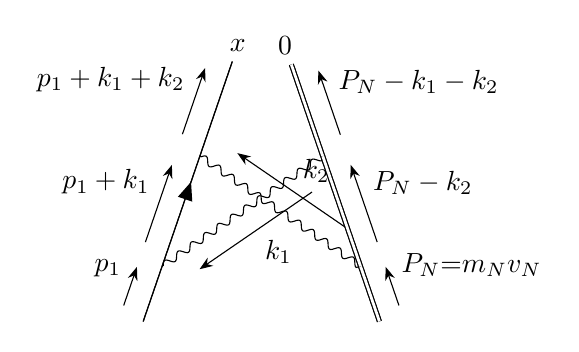
\begin{tikzpicture}[baseline=($(p1)!0.5!(x)$)]
 \begin{feynman}
    \vertex (p1);
 \vertex[right=3cm of p1] (p2);
 \vertex at ($(p1)!0.4!(p2)+(0,3.5cm)$) (x) {$x$};
 \vertex at ($(p1)!0.6!(p2)+(0,3.5cm)$) (0) {$0$};
 \vertex at ($(p1)!0.2!(x)$) (y1);
 \vertex at ($(p2)!0.2!(0)$) (z1);
 \vertex at ($(p1)!0.6!(x)$) (y2);
 \vertex at ($(p2)!0.6!(0)$) (z2);
 %
 \diagram* {
   (p1) -- [fermion] (x);
   (p2) -- [double distance=1pt] (0);
   (y1) -- [photon,rmomentum'=$k_1$] (z2);
   (y2) -- [photon,rmomentum={[distance=-3pt]$k_2$}] (z1);
   (p1) -- [momentum=\(p_{1}\)] (y1);
   (p2) -- [momentum'=$P_{N}\text{=}m_{N}v_{N}$,double distance=1pt] (z1);
   (y1) -- [momentum=\(p_{1}+k_1\)] (y2);
   (z1) -- [momentum'=\(P_{N}-k_2\),double distance=1pt] (z2);
   (y2) -- [momentum=\(p_{1}+k_1+k_2\)] (x);
   (z2) -- [momentum'=\(P_{N}-k_1-k_2\),double distance=1pt] (0);
    };
 \end{feynman}
  \end{tikzpicture}\\
  =&e^4\int[dk_1][dk_2]e^{-i\vb{(p_1+k_1+k_2)}\vdot \vb{x}}\frac{1}{\vb{\abs{k_1}}^2}\frac{1}{\vb{\abs{k_2}}^2}\frac{1}{-k_1^0-k_2^0+i\epsilon}\frac{1}{-k_2^0+i\epsilon}\frac{\slashed p_1+\slashed k_1+\slashed k_2+m}{(p_1+ k_1+ k_2)^2-m^2+i\epsilon}\g^0\frac{\slashed p_1+\slashed k_1+m}{(p_1+ k_1)^2-m^2+i\epsilon}\g^0u_N(v_N)u_e(p_1)\\
  =&e^4\int[dk_1][dk_2]e^{-i\vb{(p_1+k_1+k_2)}\vdot \vb{x}}\frac{1}{\vb{\abs{k_1}}^2\vb{\abs{k_2}}^2}
  \frac{4{p_1^0}^2+2p_1^0k_1^0+2\vb{p_1}\cdot\vb{k_1}+2(p_1^0+k_1^0)(\slashed k_1+\slashed k_2)\g^0-\slashed k_2\slashed k_1}{\bqty{(p_1+ k_1+ k_2)^2-m^2+i\epsilon}\bqty{(p_1+ k_1)^2-m^2+i\epsilon}\bqty{-k_1^0-k_2^0+i\epsilon}\bqty{-k_2^0+i\epsilon}}
  u_N(v_N)u_e(p_1)\\
  =&ie^4\int[\dd k_1]\frac{\dd^3\vb{k_2}}{(2\pi)^3}
  \frac{2(k_1^0+p_1^0)[b+\slashed k_1\g^0]-\g^0b\slashed k_1}{2\sqrt{a_2}(\sqrt{a_2}-k_1^0+i \epsilon )}
  \frac{1}{k_1^0+p_1^0-\sqrt{a_2}+\frac{i \epsilon }{2 \sqrt{a_2}}+i\epsilon}\frac{1}{(p_1+ k_1)^2-m^2+i\epsilon}\frac{1}{\vb{\abs{k_1}}^2\vb{\abs{k_2}}^2}u_N(v_N)u_e(p_1)e^{-i\vb{(p_1+k_1+k_2)}\vdot \vb{x}}\\
  =&e^4\int\frac{\dd^3\vb{k_1}}{(2\pi)^3}\frac{\dd^3\vb{k_2}}{(2\pi)^3}
  \frac{2\sqrt{a_1}(b'+k_1^i\g_i\g^0)+\g^0(\sqrt{a_1}-b'-p_1^0)(\sqrt{a_1}\g^0-p_1^0\g^0+k_1^i\g_i)}{4 \sqrt{a_1} \sqrt{a_2} \left(\sqrt{a_1}+\sqrt{a_2}\right) \left(\sqrt{a_2}-p_1^0\right)}
  \frac{1}{\vb{\abs{k_1}}^2\vb{\abs{k_2}}^2}u_N(v_N)u_e(p_1)e^{-i\vb{(p_1+k_1+k_2)}\vdot \vb{x}}\\
\end{align*}
For NRQED case ($\mel{0}{\psi_e(0)N(0)e\int\dd^4y_1\bar\psi_e\psi_e A^0e\int\dd^4z_1\bar NNA^0e\int\dd^4y_2\bar\psi_e\psi_e A^0e\int\dd^4z_2\bar NNA^0}{eN}$)
\begin{align*}
  &-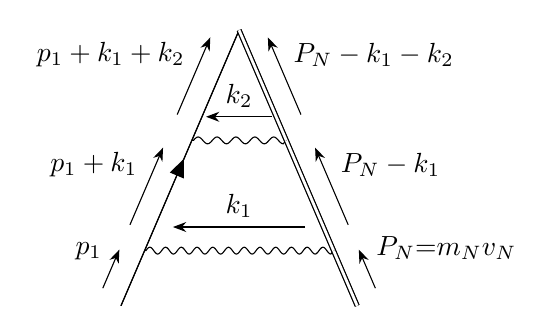
\begin{tikzpicture}[baseline=($(p1)!0.5!(x)$)]
 \begin{feynman}
   \vertex (p1);
 \vertex[right=3cm of p1] (p2);
 \vertex at ($(p1)!0.5!(p2)+(0,3.5cm)$) (x) ;
 \vertex at ($(p1)!0.2!(x)$) (y1);
 \vertex at ($(p2)!0.2!(x)$) (z1);
 \vertex at ($(p1)!0.6!(x)$) (y2);
 \vertex at ($(p2)!0.6!(x)$) (z2);
 %
 \diagram* {
   (p1) -- [fermion] (x);
   (p2) -- [double distance=1pt] (x);
   (y1) -- [photon,rmomentum=$k_1$] (z1);
   (y2) -- [photon,rmomentum=$k_2$] (z2);
   (p1) -- [momentum=\(p_{1}\)] (y1);
   (p2) -- [momentum'=$P_{N}\text{=}m_{N}v_{N}$,double distance=1pt] (z1);
   (y1) -- [momentum=\(p_{1}+k_1\)] (y2);
   (z1) -- [momentum'=\(P_{N}-k_1\),double distance=1pt] (z2);
   (y2) -- [momentum=\(p_{1}+k_1+k_2\)] (x);
   (z2) -- [momentum'=\(P_{N}-k_1-k_2\),double distance=1pt] (x);
   };
 \end{feynman}
 \end{tikzpicture}\\
 =&e^4\int[dk_1][dk_2]\frac{1}{\vb{\abs{k_1}}^2}\frac{1}{\vb{\abs{k_2}}^2}\frac{1}{-k_1^0-k_2^0+i\epsilon}\frac{1}{-k_1^0+i\epsilon}\frac{1}{p_1^0+k_1^0-m-\frac{\vb{(p_1+k_1)}^2}{2m}+i\epsilon}\frac{1}{p_1^0+k_1^0+k_2^0-m-\frac{\vb{(p_1+k_1+k_2)}^2}{2m}+i\epsilon}\psi_e(p_1)u_N(v_N)\footnotemark\\
 =&ie^4\int[dk_1]\frac{\dd^3\vb{k_2}}{(2\pi)^3}\frac{1}{\vb{\abs{k_1}}^2}\frac{1}{\vb{\abs{k_2}}^2}\frac{1}{-k_1^0+i\epsilon}\frac{1}{p_1^0+k_1^0-m-\frac{\vb{(p_1+k_1)}^2}{2m}+i\epsilon}\frac{1}{p_1^0-m-\frac{\vb{(p_1+k_1+k_2)}^2}{2m}+2i\epsilon}\psi_e(p_1)u_N(v_N)\\
 =&-e^4\int\frac{\dd^3\vb{k_1}}{(2\pi)^3}\frac{\dd^3\vb{k_2}}{(2\pi)^3}\frac{1}{\vb{\abs{k_1}}^2}\frac{1}{\vb{\abs{k_2}}^2}\frac{1}{p_1^0-m-\frac{\vb{(p_1+k_1)}^2}{2m}+2i\epsilon}\frac{1}{p_1^0-m-\frac{\vb{(p_1+k_1+k_2)}^2}{2m}+2i\epsilon}\psi_e(p_1)u_N(v_N)\\
 \intertext{do the shift as above}
 =&-e^4\int\frac{\dd^3\vb{k_1}}{(2\pi)^3}\frac{\dd^3\vb{k_2}}{(2\pi)^3}\frac{1}{\vb{\abs{k_1-p_1}}^2}\frac{1}{\vb{\abs{k_2-k_1}}^2}\frac{1}{p_1^0-m-\frac{\vb{\abs{k_1}}^2}{2m}+2i\epsilon}\frac{1}{p_1^0-m-\frac{\vb{\abs{k_2}}^2}{2m}+2i\epsilon}\psi_e(p_1)u_N(v_N)\\
 \intertext{drop $\vb{p_1}$}
 =&-e^4\int\frac{\dd^3\vb{k_1}}{(2\pi)^3}\frac{\dd^3\vb{k_2}}{(2\pi)^3}\frac{1}{\vb{\abs{k_1}}^2}\frac{1}{\vb{\abs{k_2-k_1}}^2}\frac{1}{-\frac{\vb{\abs{k_1}}^2}{2m}+2i\epsilon}\frac{1}{-\frac{\vb{\abs{k_2}}^2}{2m}+2i\epsilon}\psi_e(p_1)u_N(v_N)
\end{align*}
\footnotetext{Clearly in this line, if this NRQCD diagram is crossed, the second pole would become $-k_2^0+i \epsilon$ and the whole formula is zero (since both poles of $k_1^0$ would be in the same side).}
 \section{HSET}
 \subsection{Lagrangian}
For scalar QED
$$\mathcal{L}=(D_{\mu}\phi)^{\dagger}D^{\mu}\phi-m^2\phi^{\dagger}\phi$$
where
$$D_{\mu}=\partial_{\mu}+ieA_{\mu}$$
In Schwartz's QFT (Chap. 35) he mentioned a choice of $\chi_v$ and $\tilde \chi_v$:
\begin{align}
\phi(x)=e^{-imv\cdot x}\frac{1}{\sqrt{2m}}(\chi_v(x)+\tilde\chi_v(x))
\label{scalar}
\end{align}
\begin{align}
\chi_v(x)=e^{imv\cdot x}\frac{1}{\sqrt{2m}}(iv\cdot D+m)\phi(x),\;
\tilde\chi_v(x)=e^{imv\cdot x}\frac{1}{\sqrt{2m}}(-iv\cdot D+m)\phi(x)
\label{scalar redefine}
\end{align}
Put \eqref{scalar} into \eqref{scalar redefine}, a simple relation is derived:
$$(-iv\cdot D)\chi_v(x)=(2m+iv\cdot D)\tilde\chi_v(x)$$
It can also be writen as
$$2m\tilde\chi_v=(-iv\cdot D)(\chi_v+\tilde\chi_v) $$
Use this result
\begin{align*}
  \mathcal{L}&=\frac{1}{2m}\Big\{\Bqty{[D^{\mu}(\chi_v+\tilde\chi_v)]^{\dagger}+imv^{\mu}(\chi_v+\tilde\chi_v)^{\dagger}}\Bqty{[D_{\mu}(\chi_v+\tilde\chi_v)]-imv_{\mu}(\chi_v+\tilde\chi_v)}-m^2(\chi_v+\tilde\chi_v)^{\dagger}(\chi_v+\tilde\chi_v)\Big\}\\
  &=(\chi_v+\tilde\chi_v)^{\dagger}(iv\cdot D)(\chi_v+\tilde\chi_v)+\frac{1}{2m}[D^{\mu}(\chi_v+\tilde\chi_v)]^{\dagger}D_{\mu}(\chi_v+\tilde\chi_v)
  \stepcounter{equation}\tag{\theequation}\label{lag0}\\
&=(\chi_v(x)+\tilde\chi_v(x))^{\dagger}(iv\cdot D)(\chi_v(x)+\tilde\chi_v(x))+\mathcal{O}(\frac{1}{m}) \stepcounter{equation}\tag{\theequation}\label{lag1}
\end{align*}
(note that $D_{\mu}\phi=e^{-imv\cdot x}[D_{\mu}(\chi_v+\tilde \chi_v)-imv_{\mu}(\chi_v+\tilde\chi_v)]$ and $-imv^{\mu}[D_{\mu}(\chi_v+\tilde \chi_v)]^{\dagger}(\chi_v+\tilde \chi_v)=imv^{\mu}(\chi_v+\tilde\chi_v)^{\dagger}D_{\mu}(\chi_v+\tilde \chi_v)-total\ derivative\ term$)

Use the leading order of \eqref{lag0}
\begin{align*}
  \lag^{(0)}&=(\chi_v+\tilde\chi_v)^{\dagger}(iv\cdot D)(\chi_v+\tilde\chi_v)\\
  &=\chi_v^{\dagger}iv\cdot D\chi_v+\tilde\chi_v^{\dagger}iv\cdot D(\chi_v+\tilde\chi_v)+\chi_v^{\dagger}iv\cdot D\tilde\chi_v\\
  &=\chi_v^{\dagger}iv\cdot D\chi_v-2m\tilde\chi_v^{\dagger}\tilde\chi_v+(iv\cdot D\chi_v)^{\dagger}\tilde\chi_v\\
&=\chi_v^{\dagger}iv\cdot D\chi_v-2m\tilde\chi_v^{\dagger}\tilde\chi_v+[(-2m-iv\cdot D)\tilde\chi_v]^{\dagger}\tilde\chi_v\\
&=\chi_v^{\dagger}iv\cdot D\chi_v-\tilde\chi_v^{\dagger}(iv\cdot D+4m)\tilde\chi_v
\end{align*}

We can have the final form\footnote{With one problem: if we can tolerate coupled particle-anti particle pair, we can trade $iv\cdot D $ for mass term, so the leading part is the same but the anti-particle part could be different with the mixing? }
$$\mathcal{L}=\chi_v^{\dagger}iv\cdot D\chi_v-\tilde \chi_v^{\dagger}(iv\cdot D+4m)\tilde\chi_v+\mathcal{O}(\frac{1}{m})$$
\subsection{Quantization}
\subsubsection{HQET as an example}
The leading term of HQET Lagrangian is
\begin{align*}
  \lag=\bar Q_v(iv\cdot D)Q_v
\end{align*}
\begin{align*}
  Q_v(x)=e^{imv\cdot x}\frac{1+\slashed v}{2}\psi(x)
\end{align*}
In free Dirac fermion theory we know that
\begin{align*}
    \Bqty{\psi_a(\vb{x}),\psi_b^{\dagger}(\vb{y})}=\delta^{(3)}(\vb{x}-\vb{y})\delta_{ab}\\
	\{a_{\vb{p}},a_{\vb{p'}}^{\dagger}\}=(2\pi)^3\delta^{(3)}(\vb{p-p'})
\end{align*}
also the plane wave expansion of $\psi$ is
\begin{align*}
  \psi(x)&=\int\frac{\dd^3p}{(2\pi)^3}\frac{1}{\sqrt{2E_p}}a_{\vb{p}}u(p)e^{-ip\cdot x}\\
  &=\int \frac{\dd^3k}{(2\pi)^3}\frac{1}{\sqrt{2mv^0}}a_v\sqrt{m}u(v)e^{-imv\cdot x-ik\cdot x}\\
  \intertext{using normalization of states $u(k)=\sqrt{m}u(v)$\footnotemark, $\braket{p'}{p}=2E_p(2\pi)^3 \delta^{(3)}(\vb{p'-p})$ and $\braket{v',k'}{v,k}=2v^0\delta_{vv'}(2\pi)^3 \delta^{(3)}(\vb{k'-k})$ we have $\ket{p}=\sqrt{m}\ket{v}$ ($\ket{p}=\sqrt{2E_p}a_{\vb{p}}^{\dagger}\ket{0}$ while $\ket{v,k}=\sqrt{2v^0}a_{v,\vb{k}}^{\dagger}\ket{0}$)}
  &=\int \frac{\dd^3k}{(2\pi)^3}\frac{1}{\sqrt{2v^0}}a_vu(v)e^{-imv\cdot x-ik\cdot x}
\end{align*}
\footnotetext{The relation $\bar u^s(p)\gm u^s(p)=2p^{\mu}$ can be derived using Gordon identity, same for $\bar u^s(v)\gm u^s(v)=2v^{\mu}$, but it's actually $\bar u u$.}
Using the definition of $ Q_v(x)$
\begin{align*}
  Q_v(x)&=e^{imv\cdot x}\frac{1+\slashed v}{2}\psi(x)\\
  &=\int \frac{\dd^3k}{(2\pi)^3}\frac{1}{\sqrt{2v^0}}a_v \frac{1+\slashed v}{2}u(v)e^{-ik\cdot x}\\
  &=\int \frac{\dd^3k}{(2\pi)^3}\frac{1}{\sqrt{2v^0}}a_v u(v)e^{-ik\cdot x}
\end{align*}
The commutation relation should be
\begin{align*}
  \{Q_{va}(\vb{x}),Q_{v'b}(\vb{x'})\}&=\int \frac{\dd^3k}{(2\pi)^3}\frac{\dd^3k'}{(2\pi)^3}\frac{1}{\sqrt{4v^0v'^0}}\{a_v,a_{v'}^{\dagger}\}u_a(v)u_b^{\dagger}(v')e^{-ik\cdot x+ik'\cdot x'}\\
  \intertext{
  using $\sum_s u_a(v)u_b^{\dagger}(v)=\frac{1}{m}\sum_s u_a(p)u^{\dagger}_b(p)=[(\slashed v+1)\g^0]_{ab}$}
  &=\int \frac{\dd^3k}{(2\pi)^3}\frac{\dd^3k'}{(2\pi)^3}\frac{1}{\sqrt{4v^0v'^0}}\{a_v,a_{v'}^{\dagger}\}[(\slashed v+1)\g^0]_{ab}e^{-ik\cdot x+ik'\cdot x'}\\
  \intertext{assuming $\{a_v,a_{v'}\}=(2\pi)^3\delta_{vv'}\delta^{(3)}(\vb{k-k'})$}
  &=\int \frac{\dd^3k}{(2\pi)^3}\frac{1}{2v^0}[(\slashed v+1)\g^0]_{ab}e^{-ik\cdot (x-x')}\delta_{vv'}\\
  &=[\frac{(\slashed v+1)\g^0}{2v^0}]_{ab}\delta_{vv'}\delta^{(3)}(\vb{x-x'})
\end{align*}
\subsubsection{HSET}
The anti-particle field is decoupled so we don't have to consider that for now. The equation-of-motion is
\begin{align*}
  \begin{cases}
	v\cdot D\chi_v^{\dagger}=0\\
	v\cdot D\chi_v=0
  \end{cases}
\end{align*}
By definition
\begin{align*}
  \chi_v(x)&=\frac{e^{imv\cdot x}}{\sqrt{2m}}(iv\cdot D+m)\phi(x)\\
  &=\frac{1}{\sqrt{2m}}(iv\cdot D+2m)e^{imv\cdot x}\phi(x)
\end{align*}


\end{document}
